%%%%%%%%%%%%%%%%%%%%%%%%%%%%%%%%%%%%%%%%%%%%%%%%%%%%%%%%%%%

\chapter{Template comandi}
\label{chp:templateComandi}

Questo è un capitolo provvisorio, sarà mostrato nel documento soltanto fino al completamento del lavoro sulla documentazione. Qui di seguito è possibile trovare i template per i comandi, ad esempio i comandi per inserire tabelle, immagini, riferimenti incrociati, ecc\dots

\section{Tabelle casi d'uso}

\subsection{Tabella due attori}

Per il template della tabella dei casi d'uso con due attori, vedi la Figura \vref{tab:template-tab-casiduso-due-attori}.

\begin{table}[tb]
%\normalsize % Dimensione testo normale
\small % Dimensione testo piccola
%\footnotesize % Dimensione testo piccolissima
%\scriptsize % Dimensione del testo ulteriormente più piccola
\caption{Template tabella casi d'uso con due attori} % Didascalia tabella
\label{tab:template-tab-casiduso-due-attori} % Etichetta per riferimenti incrociati
\begin{tabular}{| p{\useCaseLeft} | p{\useCaseNum} | p{\useCaseTwoCol} | p{\useCaseTwoCol} |}
	\hline
	\textbf{Nome caso d'uso} & \multicolumn{3}{p{\useCaseMulticol} |}{\textbf{Login}} \\
	\hline
	\textbf{Attori partecipanti} & \multicolumn{3}{p{\useCaseMulticol} |}{Inizializzato da \textbf{Utente}.} \\
	\hline
	\textbf{Condizioni d'ingresso} & \multicolumn{3}{p{\useCaseMulticol} |}{L'utente ha cliccato sul bottone di login.} \\
	\hline
	\textbf{Flusso degli eventi} & \textbf{\#} & \textbf{Utente} & \textbf{Sistema} \\
	\hline
	\textbf{} & \textbf{1} & \textbf{} & Propone una schermata per l'inserimento dei dati necessari per il login, e-mail e password dell'utente \\
	\hline
	\textbf{} & \textbf{2} & Inserisce i dati e sottomette la richiesta & \textbf{} \\
	\hline
	\textbf{} & \textbf{3} & \textbf{} & Controlla che siano stati inseriti entrambi i campi e avvia le operazioni di visualizzazione \\
	\hline
	\textbf{Eccezioni} & \multicolumn{3}{p{\useCaseMulticol} |}{3.1 Uno o entrambi i campi sono vuoti.\newline 3.2 Le credenziali inserite non sono valide (una o entrambe).} \\
	\hline
	\textbf{Condizioni d'uscita} & \multicolumn{3}{p{\useCaseMulticol} |}{Il sistema completa la login e dà accesso all'app o, in caso contrario, visualizza un messaggio di errore se non sono stati inseriti tutti i dati obbligatori, se le credenziali non sono corrette o se si verifica un insuccesso dell'operazione.} \\
	\hline
\end{tabular}
\end{table}

\subsection{Tabella tre attori}

Per il template della tabella dei casi d'uso con tre attori, vedi la Figura \vref{tab:template-tab-casiduso-tre-attori}.

\begin{table}[tb]
%\normalsize % Dimensione testo normale
\small % Dimensione testo piccola
%\footnotesize % Dimensione testo piccolissima
%\scriptsize % Dimensione del testo ulteriormente più piccola
\caption{Template tabella casi d'uso con tre attori} % Didascalia tabella
\label{tab:template-tab-casiduso-tre-attori} % Etichetta per riferimenti incrociati
\begin{tabular}{| p{\useCaseLeft} | p{\useCaseNum} | p{\useCaseThreeCol} | p{\useCaseThreeCol} | p{\useCaseThreeCol} |}
	\hline
	\textbf{Nome caso d'uso} & \multicolumn{4}{p{\useCaseMulticol} |}{\textbf{Login}} \\
	\hline
	\textbf{Attori partecipanti} & \multicolumn{4}{p{\useCaseMulticol} |}{Inizializzato da \textbf{Utente}.} \\
	\hline
	\textbf{Condizioni d'ingresso} & \multicolumn{4}{p{\useCaseMulticol} |}{L'utente ha cliccato sul bottone di login.} \\
	\hline
	\textbf{Flusso degli eventi} & \textbf{\#} & \textbf{Utente} & \textbf{Sistema} & \textbf{Attore 3} \\
	\hline
	\textbf{} & \textbf{1} & \textbf{} & Propone una schermata per l'inserimento dei dati necessari per il login, e-mail e password dell'utente & \textbf{} \\
	\hline
	\textbf{} & \textbf{2} & Inserisce i dati e sottomette la richiesta & \textbf{} & \textbf{} \\
	\hline
	\textbf{} & \textbf{3} & \textbf{} & \textbf{} & Controlla che siano stati inseriti entrambi i campi e avvia le operazioni di visualizzazione \\
	\hline
	\textbf{Eccezioni} & \multicolumn{4}{p{\useCaseMulticol} |}{3.1 Uno o entrambi i campi sono vuoti.\newline 3.2 Le credenziali inserite non sono valide (una o entrambe).} \\
	\hline
	\textbf{Condizioni d'uscita} & \multicolumn{4}{p{\useCaseMulticol} |}{Il sistema completa la login e dà accesso all'app o, in caso contrario, visualizza un messaggio di errore se non sono stati inseriti tutti i dati obbligatori, se le credenziali non sono corrette o se si verifica un insuccesso dell'operazione.} \\
	\hline
\end{tabular}
\end{table}

\subsection{Tabella quattro attori}

Per il template della tabella dei casi d'uso con quattro attori, vedi la Figura \vref{tab:template-tab-casiduso-quattro-attori}.

\begin{table}[tb]
%\normalsize % Dimensione testo normale
%\small % Dimensione testo piccola
\footnotesize % Dimensione testo piccolissima
%\scriptsize % Dimensione del testo ulteriormente più piccola
\caption{Template tabella casi d'uso con quattro attori} % Didascalia tabella
\label{tab:template-tab-casiduso-quattro-attori} % Etichetta per riferimenti incrociati
\begin{tabular}{| p{\useCaseLeft} | p{\useCaseNum} | p{\useCaseFourCol} | p{\useCaseFourCol} | p{\useCaseFourCol} | p{\useCaseFourCol} | }
	\hline
	\textbf{Nome caso d'uso} & \multicolumn{5}{p{\useCaseMulticol} |}{\textbf{Login}} \\
	\hline
	\textbf{Attori partecipanti} & \multicolumn{5}{p{\useCaseMulticol} |}{Inizializzato da \textbf{Utente}.} \\
	\hline
	\textbf{Condizioni d'ingresso} & \multicolumn{5}{p{\useCaseMulticol} |}{L'utente ha cliccato sul bottone di login.} \\
	\hline
	\textbf{Flusso degli eventi} & \textbf{\#} & \textbf{Utente} & \textbf{Sistema} & \textbf{Attore 3} & \textbf{Attore 4} \\
	\hline
	\textbf{} & \textbf{1} & \textbf{} & Propone una schermata per l'inserimento dei dati necessari per il login, e-mail e password dell'utente & \textbf{} & \textbf{} \\
	\hline
	\textbf{} & \textbf{2} & Inserisce i dati e sottomette la richiesta & \textbf{} & \textbf{} & \textbf{} \\
	\hline
	\textbf{} & \textbf{3} & \textbf{} & \textbf{} & Controlla che siano stati inseriti entrambi i campi e avvia le operazioni di visualizzazione & \textbf{} \\
	\hline
	\textbf{} & \textbf{4} & \textbf{} & \textbf{} & \textbf{} & Controlla che siano stati inseriti entrambi i campi e avvia le operazioni di visualizzazione \\
	\hline
	\textbf{Eccezioni} & \multicolumn{5}{p{\useCaseMulticol} |}{3.1 Uno o entrambi i campi sono vuoti.\newline 3.2 Le credenziali inserite non sono valide (una o entrambe).} \\
	\hline
	\textbf{Condizioni d'uscita} & \multicolumn{5}{p{\useCaseMulticol} |}{Il sistema completa la login e dà accesso all'app o, in caso contrario, visualizza un messaggio di errore se non sono stati inseriti tutti i dati obbligatori, se le credenziali non sono corrette o se si verifica un insuccesso dell'operazione.} \\
	\hline
\end{tabular}
\end{table}

\subsection{Tabella cinque attori}

Per il template della tabella dei casi d'uso con cinque attori, vedi la Figura \vref{tab:template-tab-casiduso-cinque-attori}.

\begin{table}[tb]
%\normalsize % Dimensione testo normale
%\small % Dimensione testo piccola
\footnotesize % Dimensione testo piccolissima
%\scriptsize % Dimensione del testo ulteriormente più piccola
\caption{Template tabella casi d'uso con cinque attori} % Didascalia tabella
\label{tab:template-tab-casiduso-cinque-attori} % Etichetta per riferimenti incrociati
\begin{tabular}{| p{\useCaseLeft} | p{\useCaseNum} | p{\useCaseFiveCol} | p{\useCaseFiveCol} | p{\useCaseFiveCol} | p{\useCaseFiveCol} | p{\useCaseFiveCol} | }
	\hline
	\textbf{Nome caso d'uso} & \multicolumn{6}{p{\useCaseMulticol} |}{\textbf{Login}} \\
	\hline
	\textbf{Attori partecipanti} & \multicolumn{6}{p{\useCaseMulticol} |}{Inizializzato da \textbf{Utente}.} \\
	\hline
	\textbf{Condizioni d'ingresso} & \multicolumn{6}{p{\useCaseMulticol} |}{L'utente ha cliccato sul bottone di login.} \\
	\hline
	\textbf{Flusso degli eventi} & \textbf{\#} & \textbf{Utente} & \textbf{Sistema} & \textbf{Attore 3} & \textbf{Attore 4} & \textbf{Attore 5} \\
	\hline
	\textbf{} & \textbf{1} & \textbf{} & Propone una schermata per l'inserimento dei dati necessari per il login, e-mail e password dell'utente & \textbf{} & \textbf{} & \textbf{} \\
	\hline
	\textbf{} & \textbf{2} & Inserisce i dati e sottomette la richiesta & \textbf{} & \textbf{} & \textbf{} & \textbf{} \\
	\hline
	\textbf{} & \textbf{3} & \textbf{} & \textbf{} & Controlla che siano stati inseriti entrambi i campi e avvia le operazioni di visualizzazione & \textbf{} & \textbf{} \\
	\hline
	\textbf{} & \textbf{4} & \textbf{} & \textbf{} & \textbf{} & Inserisce i dati e sottomette la richiesta & \textbf{} \\
	\hline
	\textbf{} & \textbf{5} & \textbf{} & \textbf{} & \textbf{} & \textbf{} & Inserisce i dati e sottomette la richiesta \\
	\hline
	\textbf{Eccezioni} & \multicolumn{6}{p{\useCaseMulticol} |}{3.1 Uno o entrambi i campi sono vuoti.\newline 3.2 Le credenziali inserite non sono valide (una o entrambe).} \\
	\hline
	\textbf{Condizioni d'uscita} & \multicolumn{6}{p{\useCaseMulticol} |}{Il sistema completa la login e dà accesso all'app o, in caso contrario, visualizza un messaggio di errore se non sono stati inseriti tutti i dati obbligatori, se le credenziali non sono corrette o se si verifica un insuccesso dell'operazione.} \\
	\hline
\end{tabular}
\end{table}

\section{Immagini (sia raster che vettoriali)}

Per il template del comando di inserimento delle immagini (raster, vettoriali, pdf), vedi la Figura \vref{fig:template-inserimento-immagine}.

\LaTeX\ per impostazione predefinita non permette di selezionare il punto esatto in cui posizionare l'immagine. Questo perché \LaTeX\ applica un complesso algoritmo per posizionare testo e immagini in modo da seguire le norme tipografiche e produrre un documento di qualità. Non forzate il posizionamento delle immagini in un punto preciso: fidatevi di \LaTeX , conosce le norme tipografiche meglio di noi!

Quando avete bisogno di riferirvi ad una figura, usate i riferimenti incrociati, che vi permettono di indicare numero della figura e pagina dove la figura si trova, come nel seguente esempio: vedi Figura \vref{fig:template-inserimento-immagine}. Il comando usato per inserire riferimenti incrociati è \verb!\vref{}!: l'argomento di questo comando deve coincidere con l'argomento del comando \verb!\label{}! della figura a cui si vuole puntare: in tal modo \verb!\vref{}! sa a chi deve far riferimento.

In alternativa a \verb!\vref{}! potete usare il comando \verb!\ref{}!, che stampa solo il numero della figura ma non la pagina, come in questo esempio: Figura \ref{fig:template-inserimento-immagine}.

Potete regolare la larghezza delle immagini: nei comandi di inserimento della Figura \ref{fig:template-inserimento-immagine} c'è il comando \verb!\includegraphics[width=0.7\textwidth]!: questo comando imposta la larghezza dell'immagine alla larghezza del testo della pagina moltiplicata per $0,7$. È possibile modificare questo moltiplicatore, ad esempio settandolo a $0,5$, in modo da impostare la larghezza dell'immagine a metà della larghezza del testo della pagina. Non impostare mai questo parametro ad un valore superiore ad $1$, altrimenti l'immagine verrà più grande della larghezza del testo della pagina.

\begin{figure}
	\centering
	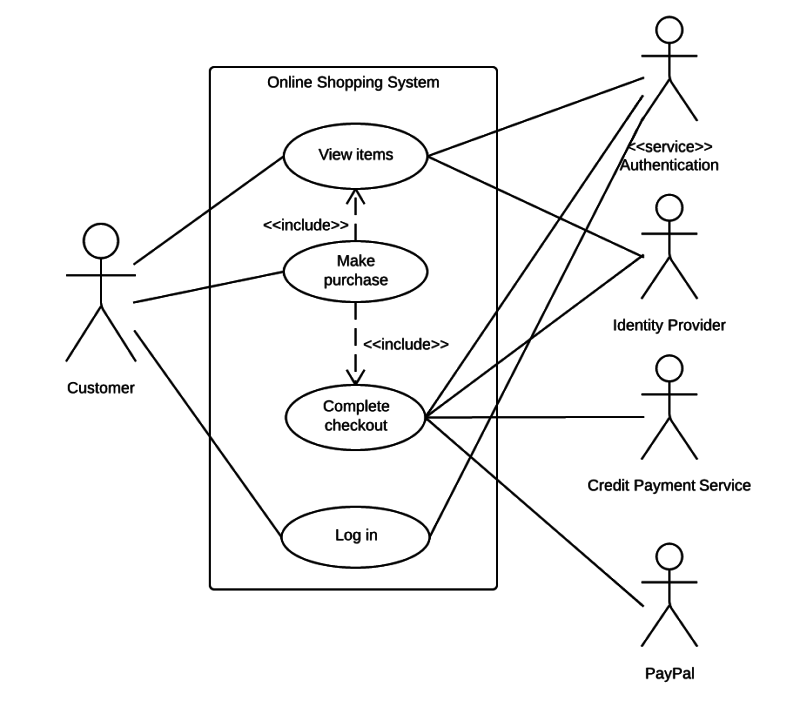
\includegraphics[width=0.7\textwidth]{imgs/file-comuni-ai-gruppi/useCaseEsempio.png}
	\caption{Template inserimento immagine}
	\label{fig:template-inserimento-immagine}
\end{figure}

\section{Punti interrogativi al posto degli indici}

Potrebbe capitarvi di compilare il documento e di vedere dei punti interrogativi in corrispondenza degli indici oppure un indice non aggiornato. In tal caso, compilate una seconda volta il documento. Questo perché \LaTeX , nella prima compilazione, calcola gli indici delle sezioni e dei riferimenti, e nella seconda compilazione integra questi indici nel documento.

\clearpage